
To reduce the background from $WZ$ and $ZZ$ processes, we veto events
containing an additional lepton satisfying the previously described selection requirements
with $\pt > 10~\GeVc$.

At the leading order $\dyll$ processes do not have $\met$. 
However $\dyll$ background contribute to the signal region due to the 
fake $\met$ arising from the jet mis-measurement. 
Therefore for those residual $\dyll$ background, the 
$\met$ is along the direction of the mis-measured jet. 
Figure~\ref{fig:dphijetmetmc} shows the the angle between the $\met$ 
and the jet that is closest to the $\met$. 
We veto events with the $\delphijetmet < 0.5$. 
This selection is only applied if the jet $\pt>15\GeVc$. 
%Figure~\ref{fig:dphidilepjet_zzpresel} shows the variable 
%$\Delta\phi(\vec{p}_{\ell}, \text{leading jet})$ in data at
%the preselection level. The Drell-Yan background is predicted
%using the method described in Section \ref{sec:bkg_dy}.

%%%%%%%%
\begin{figure}[!hbtp]
\begin{center}
\label{fig:dphijetmetmc}
\subfigure[]{
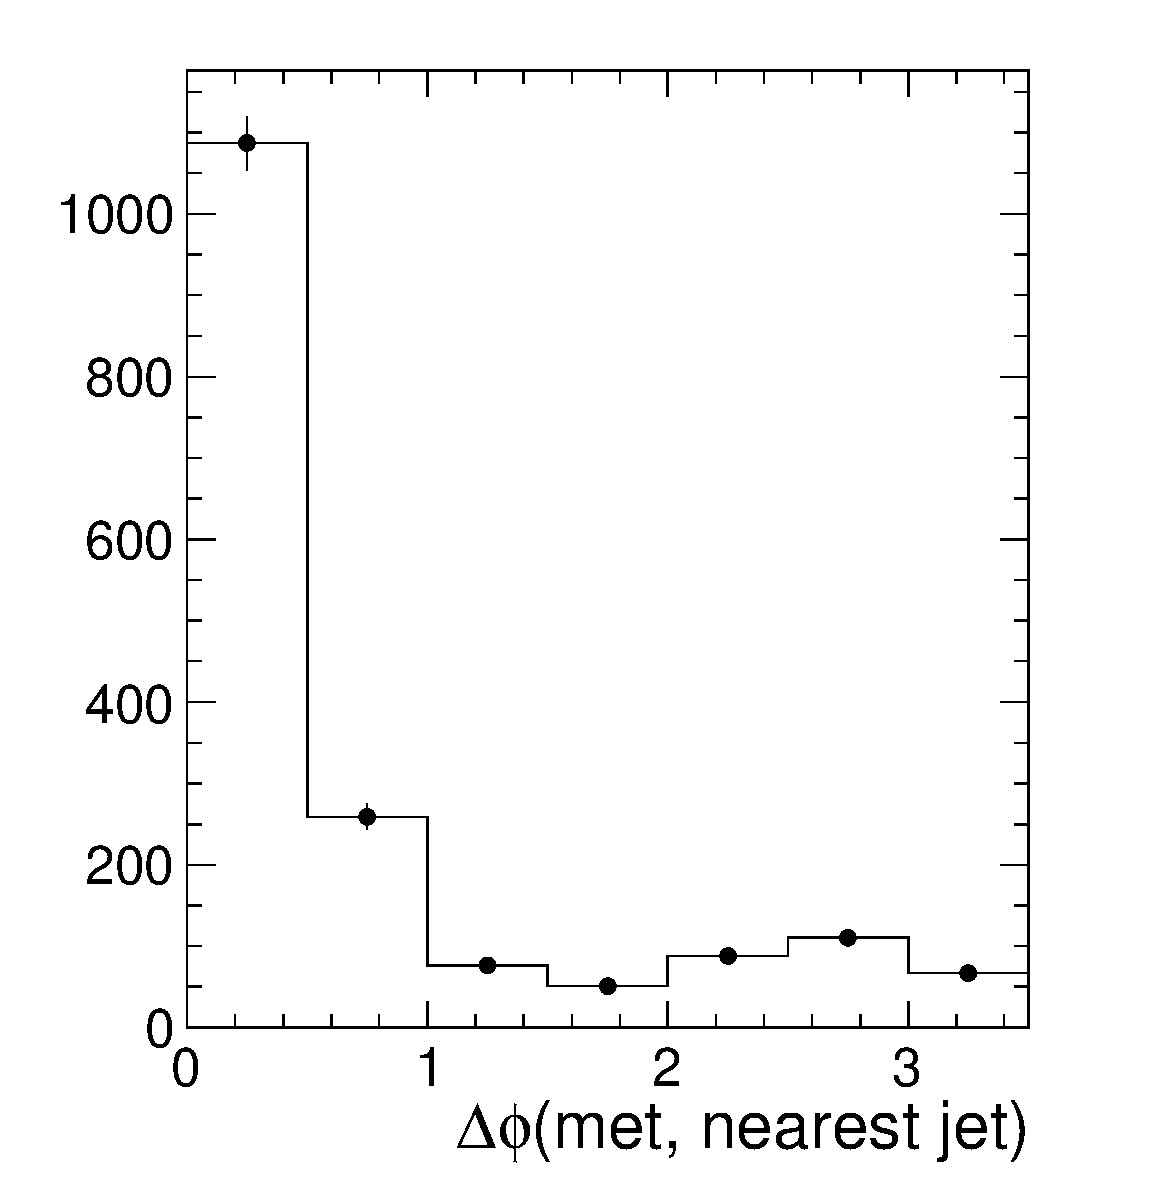
\includegraphics[width=0.5\textwidth]{figures/dphijetmet_metcut50_mc.pdf}}
\caption{The $\delphijetmet$ distribution after the other $\ZZ$ preselection requirements 
for Drell-Yan MC.}	
\end{center}
\end{figure}
%%%%%%%%




%To reject the $\dytt$ background, we require the transverse mass of the dilepton system 
%and the missing energy, 
%\begin{equation}
%M_{T}^{2} = \left( \sqrt{p_{T\mathrm{ ll}}^{2} + M_{ll}^{2}} + \sqrt{(\met)^{2} + M_{ll}^{2}} \right)^{2} - \left(\vec{p_{T\mathrm{ ll}}} + \vec{\met}\right)^{2}. \\
%\label{eq:MTHZZ}
%\end{equation}
%Figure~\ref{fig:mtemloosesel} shows the $M_T$ distribution in the $e\mu$ final state for 
%various background. The \dytt\  background has a lower $M_T$ values compared to signal. 
%Therefore we apply $M_T>150\GeV$ as part of the $\ZZ$ preselection.

%%%%%%%%%%%%%%%
%\begin{figure}[!hbtp]
%\begin{center}
%\label{fig:mtemloosesel}
%\subfigure[0-Jet]{\label{subfig:dphidilepjet_0j}
%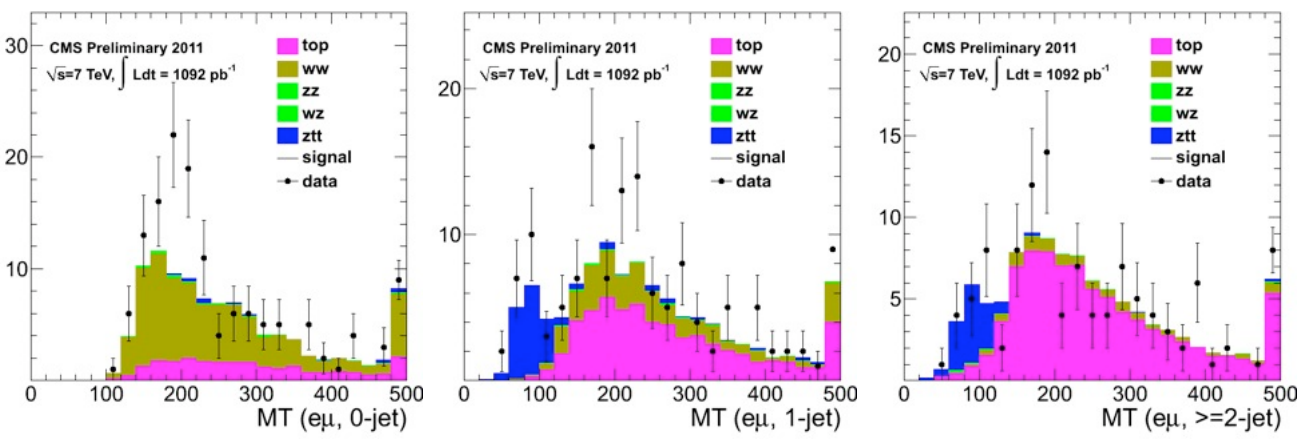
\includegraphics[width=1.0\textwidth]{figures/mtemloosemet.png}}
%\caption{\fixme\bf{replace with newer datsets and inclusive jetbins} The $M_T$ distribution in the $e\mu$ final state after the other $\ZZ$ preselection requirements.}
%\end{center}
%\end{figure}
%%%%%%%%%%%%%%%

%The expected number of signal and background events for an integrated 
%luminosity of \intlumi after applying the $\ZZ$ like selection are reported in 
%Table~\ref{tab:zzselection_all}


%To reject the Drell-Yan background due to the jet energy mismeasurement in 
%the recoiling jet, the angle between the dilepton system and the jet in 
%the transverse plane must be smaller than 165 degrees. 
%This selection is only applied if the jet $\pt>15\GeVc$. 
%Figure~\ref{fig:dphidilepjet_zzpresel} shows the variable 
%$\Delta\phi(\vec{p}_{\ell}, \text{leading jet})$ in data at
%the preselection level. The Drell-Yan background is predicted
%using the method described in Section \ref{sec:bkg_dy}.

%%%%%%%%
%\begin{figure}[!hbtp]
%\begin{center}
%\label{fig:dphidilepjet_zzpresel}
%\subfigure[0-Jet]{\label{subfig:dphidilepjet_0j}
%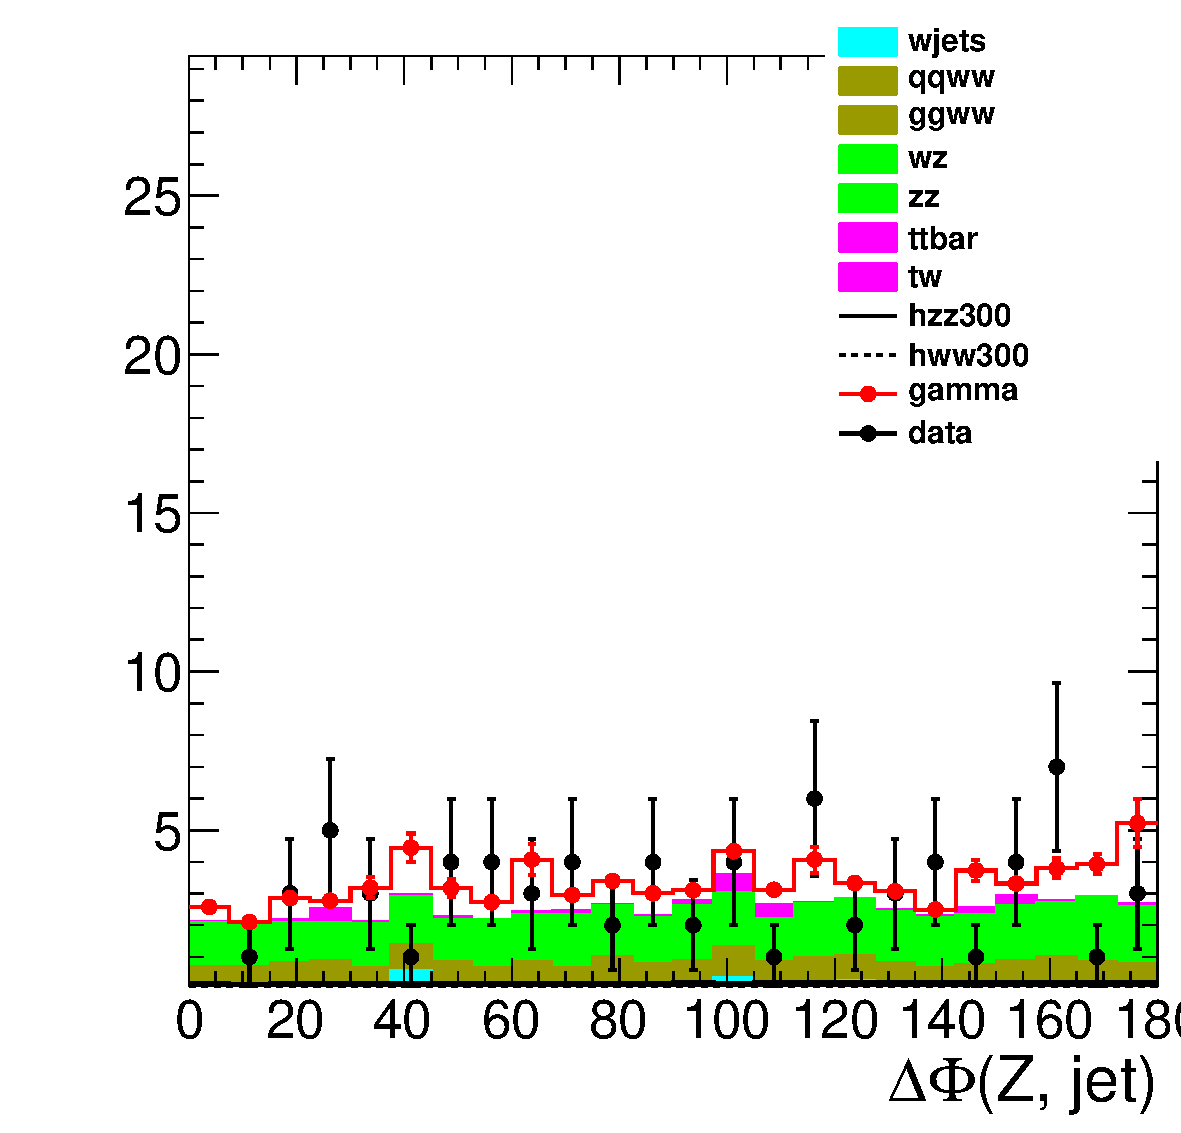
\includegraphics[width=.3\textwidth]{figures/presel_hzz300_dphidilepjet_0j.pdf}}
%\subfigure[1-Jet]{\label{subfig:dphidilepjet_1j}
%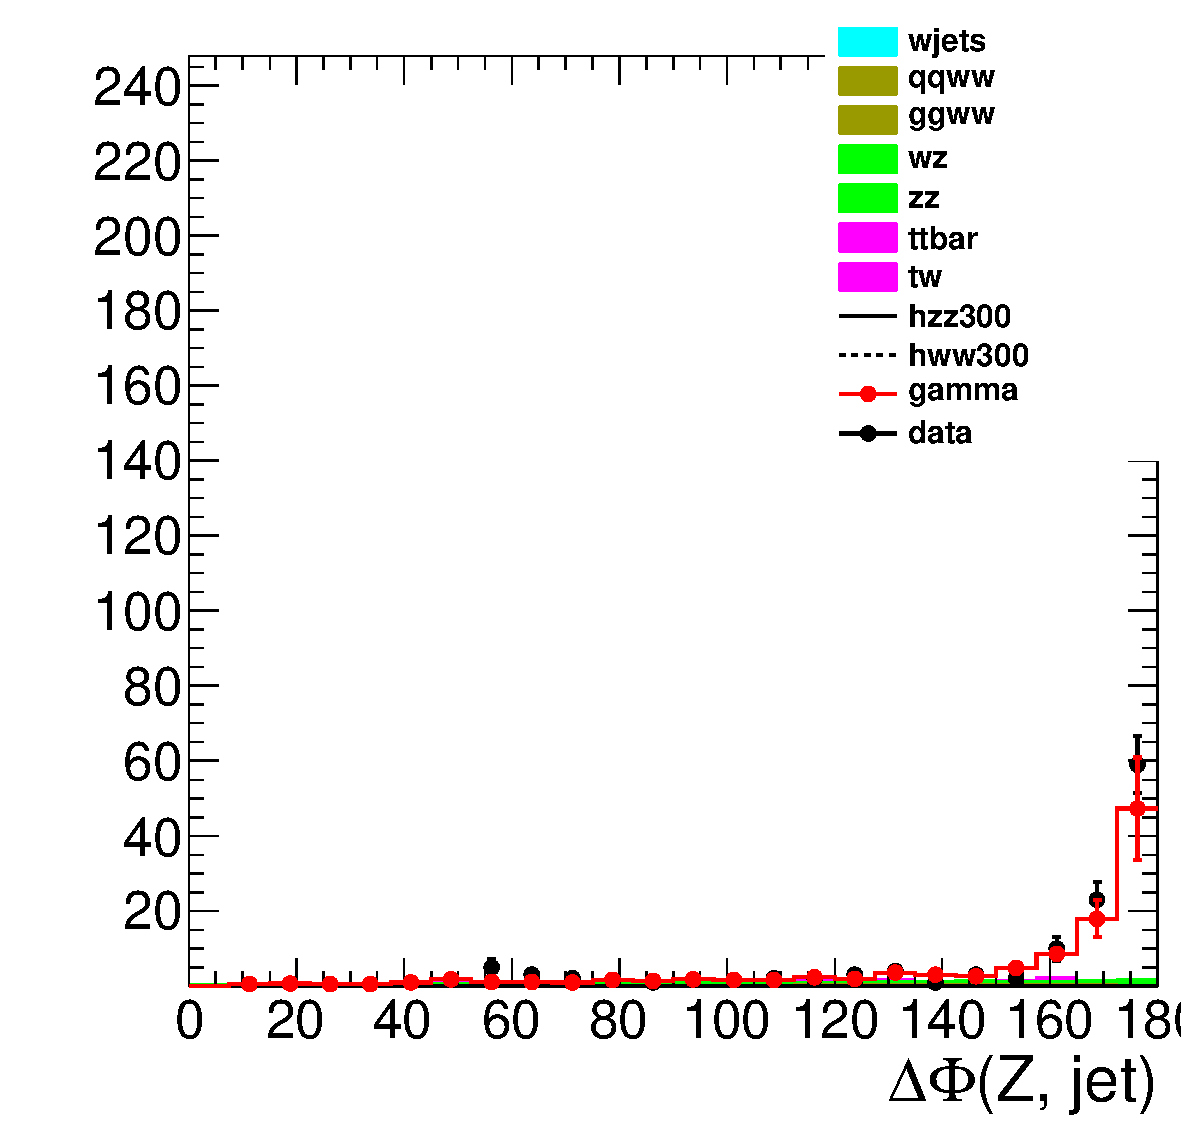
\includegraphics[width=.3\textwidth]{figures/presel_hzz300_dphidilepjet_1j.pdf}}
%\subfigure[$\geq$2 Jets]{\label{subfig:dphidilepjet_2j}
%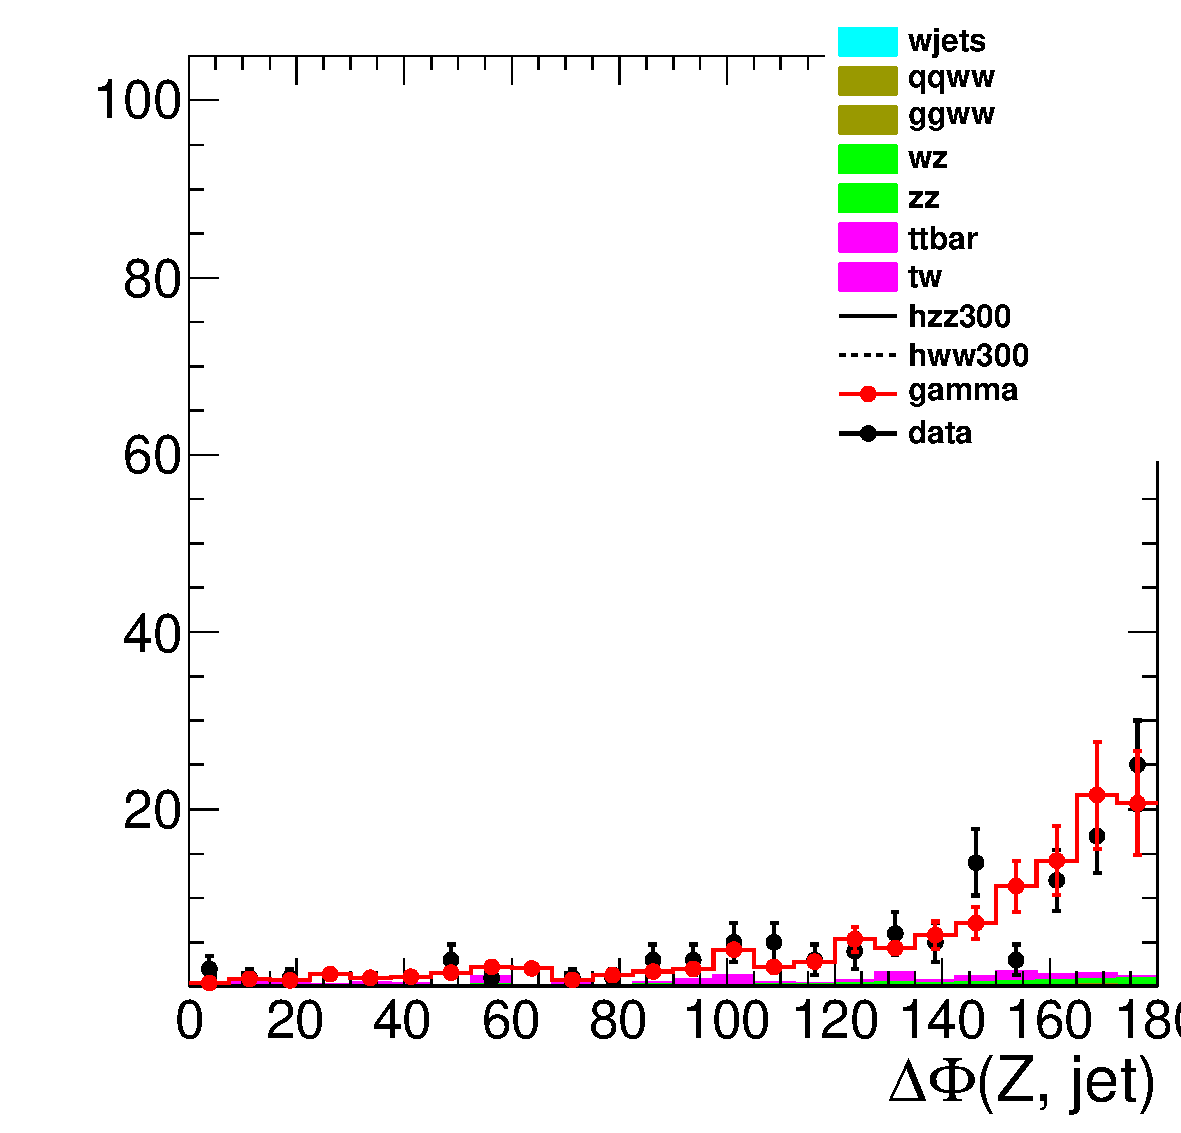
\includegraphics[width=.3\textwidth]{figures/presel_hzz300_dphidilepjet_2j.pdf}}
%\caption{$\Delta\phi(\mathrm{dilepton, leading jet})$ distribution after the other $\ZZ$ preselection requirements
%corresponding to $1092\pm7$~\ipb data in 0-Jet~\subref{subfig:dphidilepjet_0j}, 1-Jet~\subref{subfig:dphidilepjet_1j}
%and 2-Jet~\subref{subfig:dphidilepjet_2j} bins, compared to the expected from simulation for signal and background.
%The MC backgrounds are scaled as appropriate and the photon+jets estimate of the Z+jets background is added to the stack.
%In the 0-Jet and 1-Jet bins we require this to be less than 165 degrees to reduce the Z+jets background}
%\end{center}
%\end{figure}
%%%%%%%%

